\section{Answer Set Programming for explainable planning}
\subsection{Planning problem definition in FOL}
\begin{minipage}[t]{0.2\textwidth}
    \begin{figure}[H]
        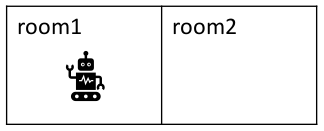
\includegraphics[width=0.9\textwidth]{img/env.png}
        \centering
    \end{figure}
\end{minipage}
\begin{minipage}[t]{0.8\textwidth}
    Given the problem on the left where a robot starting in room A has to change room.\\
    We define the knowledge base in FOL:
    \setstretch{0.5}
    \begin{itemize}
        \item Rooms A, B with possible constant values room1, room2
        \item Location (state) $at(A)$
        \item Action predicate $move(A, B)$
        \begin{itemize}
            \item Precondition: $move(A, B) \leftarrow at(A)$
            \item Effect 1 (post-cond.): $at(B) \leftarrow move(A, B)$
            \item Effect 2: $not\;at(A) \leftarrow move(A, B)$
            \item Constraint: $move(A, B),\;A \ne B$
        \end{itemize}
        \item Initial state: $at(room1)$
        \item Goal state: $at(room2)$
    \end{itemize}
\end{minipage}
\setstretch{1}
\subsubsection*{Model Checking}
To solve the problem with Model Checking we have to first enumetare all possibilites.\\
What's the plan?
\begin{itemize}
    \item Start from the initial state $at(room1)$
    \item Which variables can we substitute (ground) in $move(A, B)$?
    \begin{itemize}
        \item $move(room1, room2)$
        \item $move(room2, room1)$
        \item $move(room1, room1)$
        \item $move(room2, room2)$
    \end{itemize}
\end{itemize}

\vspace*{1pt}
Now knowing that we are $at(room1)$ we can use our \textbf{precondition} to remove actions that violates those.\\

\begin{minipage}[t]{0.5\textwidth}
    \setstretch{0.5}
    \begin{itemize}
        \item Rooms A, B with possible constant values room1, room2
        \item Location (state) $at(A)$
        \item Action predicate $move(A, B)$
        \begin{itemize}
            \item \textcolor{red}{Precondition: $move(A, B) \leftarrow at(A)$}
            \item Effect 1 (post-cond.): $at(B) \leftarrow move(A, B)$
            \item Effect 2: $not\;at(A) \leftarrow move(A, B)$
            \item Constraint: $move(A, B),\;A \ne B$
        \end{itemize}
        \item Initial state: $at(room1)$
        \item Goal state: $at(room2)$
    \end{itemize}
\end{minipage}
\begin{minipage}[t]{0.8\textwidth}
    \begin{itemize}
        \item Start from the initial state $at(room1)$
        \item Which variables can we substitute (ground) in $move(A, B)$?
        \begin{itemize}
            \item $move(room1, room2)$
            \item \textcolor{red}{\st{$move(room2, room1)$}}
            \item $move(room1, room1)$
            \item \textcolor{red}{\st{$move(room2, room2)$}}
        \end{itemize}
    \end{itemize}
\end{minipage}
\newpage
\noindent
Now knowing that we are $at(room1)$ we can use our constraint to remove actions that violates that.\\

\begin{minipage}[t]{0.5\textwidth}
    \setstretch{0.5}
    \begin{itemize}
        \item Rooms A, B with possible constant values room1, room2
        \item Location (state) $at(A)$
        \item Action predicate $move(A, B)$
        \begin{itemize}
            \item \textcolor{red}{Precondition: $move(A, B) \leftarrow at(A)$}
            \item Effect 1 (post-cond.): $at(B) \leftarrow move(A, B)$
            \item Effect 2: $not\;at(A) \leftarrow move(A, B)$
            \item \textcolor{blue}{Constraint: $move(A, B),\;A \ne B$}
        \end{itemize}
        \item Initial state: $at(room1)$
        \item Goal state: $at(room2)$
    \end{itemize}
\end{minipage}
\begin{minipage}[t]{0.8\textwidth}
    \begin{itemize}
        \item Start from the initial state $at(room1)$
        \item Which variables can we substitute (ground) in $move(A, B)$?
        \begin{itemize}
            \item $\bm{move(room1, room2)}$
            \item \textcolor{red}{\st{$move(room2, room1)$}}
            \item \textcolor{blue}{\st{$move(room1, room1)$}}
            \item \textcolor{red}{\st{$move(room2, room2)$}}
        \end{itemize}
    \end{itemize}
\end{minipage}
\setstretch{1}
\vspace{0.5cm}
Now by applying preconditions and constraints we found that the only feasible action is $move(room1, room2)$.
Progating that action we can see that we reach the goal.

\begin{minipage}[t]{0.5\textwidth}
    \setstretch{0.5}
    \begin{itemize}
        \item Rooms A, B with possible constant values room1, room2
        \item Location (state) $at(A)$
        \item Action predicate $move(A, B)$
        \begin{itemize}
            \item \textcolor{red}{Precondition: $move(A, B) \leftarrow at(A)$}
            \item \textcolor{ForestGreen}{Effect 1 (post-cond.): $at(B) \leftarrow move(A, B)$}
            \item Effect 2: $not\;at(A) \leftarrow move(A, B)$
            \item \textcolor{blue}{Constraint: $move(A, B),\;A \ne B$}
        \end{itemize}
        \item Initial state: $at(room1)$
        \item Goal state: $at(room2)$
    \end{itemize}
\end{minipage}
\begin{minipage}[t]{0.8\textwidth}
    \begin{itemize}
        \item Start from the initial state $at(room1)$
        \item Which variables can we substitute (ground) in $move(A, B)$?
        \begin{itemize}
            \item $\bm{move(room1, room2)}$
            \item \textcolor{red}{\st{$move(room2, room1)$}}
            \item \textcolor{blue}{\st{$move(room1, room1)$}}
            \item \textcolor{red}{\st{$move(room2, room2)$}}
        \end{itemize}
    \end{itemize}
\end{minipage}
\setstretch{1}
\vspace{0.1cm}

Which term may I infer? \textcolor{ForestGreen}{$at(room2)$}. This means that we reached the goal and so
$\{move(room1,room2)\}$ is a solution for this planning problem.

\subsubsection*{Absurd Reduction}
\begin{itemize}
    \item KB\footnote{KB also includes axioms, here omitted for simplicity}$=\{at(room1), \underline{at(room2)}, move(room1,room2)\}$
    \item Add goal negation: $KB + \{\underline{not\;at(room2)}\}$
\end{itemize}
Extended KB is contradictory.
Absurdum $\rightarrow \{move(room1,room2)\}$ is ground and solves the planning problem

If we continue progating with the second Effect
% What happens if we add Time?

\begin{minipage}[t]{0.5\textwidth}
    \setstretch{0.5}
    \begin{itemize}
        \item Rooms A, B with possible constant values room1, room2
        \item Location (state) $at(A)$
        \item Action predicate $move(A, B)$
        \begin{itemize}
            \item \textcolor{red}{Precondition: $move(A, B) \leftarrow at(A)$}
            \item \textcolor{ForestGreen}{Effect 1 (post-cond.): $at(B) \leftarrow move(A, B)$}
            \item \textcolor{Dandelion}{Effect 2: $not\;at(A) \leftarrow move(A, B)$}
            \item \textcolor{blue}{Constraint: $move(A, B),\;A \ne B$}
        \end{itemize}
        \item Initial state: $at(room1)$
        \item Goal state: $at(room2)$
    \end{itemize}
\end{minipage}
\begin{minipage}[t]{0.8\textwidth}
    \begin{itemize}
        \item Start from the initial state $at(room1)$
        \item Which variables can we substitute (ground) in $move(A, B)$?
        \begin{itemize}
            \item $\bm{move(room1, room2)}$
            \item \textcolor{red}{\st{$move(room2, room1)$}}
            \item \textcolor{blue}{\st{$move(room1, room1)$}}
            \item \textcolor{red}{\st{$move(room2, room2)$}}
        \end{itemize}
    \end{itemize}
\end{minipage}
\setstretch{1}

KB=$\{\underline{at(room1)}, at(room2), move(room1,room2), \underline{\textcolor{Dandelion}{not\;at(room1)}\}}$

By doing so we reach an Absurdum inside out knowledge base. Which is a problem, to solve this we need to add time.
\vspace{0.5cm}

We define the knowledge base in FOL:
\setstretch{0.5}
\begin{itemize}
    \item Rooms A, B with possible constant values room1, room2
    \item Location (state) $at(A)$
    \item Action predicate $move(A, B)$
    \begin{itemize}
        \item Precondition: $move(A, B, \textcolor{red}{t}) \leftarrow at(A, \textcolor{red}{t})$
        \item Effect 1 (post-cond.): $at(B, \textcolor{red}{t+1}) \leftarrow move(A, B, \textcolor{red}{t})$
        \item Effect 2: $not\;at(A, \textcolor{red}{t+1}) \leftarrow move(A, B, \textcolor{red}{t})$
        \item Constraint: $move(A, B, \textcolor{red}{t}),\;A \ne B$
    \end{itemize}
    \item Initial state: $at(room1, \textcolor{red}{0})$
    \item Goal state: $at(room2, \textcolor{red}{t>0})$
\end{itemize}
\setstretch{1}
With similar reasoning as above:
KB=$\{at(room1, 0), move(room1,room2, 0), not\;at(room1, 1), at(room2, 1)\}$

Resolving with Absurd Reduction: $KB + \{not\;at(room2, 1)\}$ we reach an absurdum

\subsection{Practical implementation of FOL for plan representation and reasoning}
Practical implementations of FOL and logical formalisms, to perform autonomous reasoning and inference, are logic programs.
Several options exist:
\begin{itemize}
    \item Prolog (FOL)
    \item \textbf{Answer Set Programming (FOL)}
    \item Problog (FOL + probability)
    \item Temporal ASP (FOL + LTL)
\end{itemize}
For this course we'll use Answer Set Programming (ASP).
\subsection{Answer Set Programming (ASP)}
A logic programming paradigm specifically intended for planning representation and reasoning.

It contains useful constructs fot planning:
\begin{itemize}
    \item Weak constraints (optimization)
    \item Aggregates (choice among actions)
    \item API interfaces with external programs (e.g., sensors)
    \item Non-monotonic reasoning (plan revision)
    \item Built-in time and goal representation
\end{itemize}

\subsubsection{Syntax}
Variables are marked with capital letter, constants and predicates (or atoms) with lower case.
Constants are either strings or integers.

Example: $move(A, B, T), move(room1, room2, 1)$\\

Logical implications are written with capital and minus signs (:-) with a head body structure (head :- body) 
% where the head implies the body.

Example: $move(A, B, T)$ :- $at(A, T)$\\

Logical Conjunction: is expressed with a comma or a semicolon

Example: $move(A, B, T)$ :- $at(A, T), free(B, T)$ or $move(A, B, T)$ :- $at(A, T); free(B, T)$\\

Logical negation: is expressed with a minus sing

Example: $-at(A, T+1)$ :- $move(A, B, T)$\\

Default negation: also called Negation As Failure(NAF)

Example: $not\;at(A, T+1)$ :- $move(A, B, T)$\\

\subsection{Two negations}

\begin{table}[H]
    \centering
    \begin{tabular}{cclcc}
    \multicolumn{2}{c}{{\color[HTML]{000000} \textbf{Logic Negation}}} &  & \multicolumn{2}{c}{\textbf{Negation As Failure}}             \\
    {\color[HTML]{FD6864} $p$}      & {\color[HTML]{FD6864} $-p$}      &  & {\color[HTML]{FD6864} $p$} & {\color[HTML]{FD6864} $not\;p$} \\
    0 & 1 &  & 0 & 1 \\
    1 & 0 &  & 0 & 1 \\
    ? & ? &  & ? & 0
    \end{tabular}
\end{table}

\begin{itemize}
    \item \textbf{Logic (classical or Boolean) negation}:\\
    p may be an observation, hence it may be unknown (e.g., in robotic navigation)

    \item  \textbf{Negation As Failure (NAF)}:\\
    if $p$ is unknown we set it to false by default
\end{itemize}

\textbf{Why NAF?}
Real World is characterized by Incomplete observations. If the agent does not know (observe) something, he could get stuck!
NAF allows to reason on default if a fact is unknown, assume it is false by default.

This behaviour is called \emph{Closed-World Assumption (CWA)}, this simple assumption states that if I don't know something, it is not important.\\

The planning scenario is typically dynamic (the environment may change, new observations may be acquired...).
So if we use the $CWA$ once we'll discover new information we'll update our knowledge.\\

This is possible only if the knowledge base (and related logic formalism) is \textbf{non-monotonic}.

\begin{itemize}
    \item \textbf{Monotonic KB (and formalism)}
    \begin{itemize}
        \item Given K and A, if $K \models A$ then $K \cup S \models A$ \textbf{for all S} (additional knowledge or
        rules)
    \end{itemize}
    \item \textbf{Non-monotonic KB (and formalism)}
    \begin{itemize}
        \item Given K and A, if $K \models A$ then $K \cup S \models A$ \textbf{may not hold for some S} (additional knowledge or rules)
        \item This is called Knowledge revision (dynamic knowledge)
    \end{itemize}
\end{itemize}

\subsubsection{Structure of ASP program}
In an ASP program, variables are defined like this:
\begin{itemize}
    \item Range of variables: $room(room1; room2)\quad time(1..10)$
    \item A generic room variable as an atom: $room(A)$
    \item Typically, we start an ASP program defining ranges of variables
\end{itemize}
We can also define facts, i.e., atoms with no variables
\begin{itemize}
    \item $closed\_door$
\end{itemize}

A rule, or axiom, must be safe, i.e., \textbf{all variables in the head must appear also in the body without negation nor NAF}
Examples:
\begin{itemize}
    \item $move(A, B)$ :- $not\;closed\_door, at(A)$ \cross
    \item $move(A, B)$ :- $not\;closed\_door, at(A), room(B)$ \tick
    \item $move(A, B, T)$ :- $not\;closed\_door, at(A), room(B)$ \cross
    \item $move(A, B, T)$ :- $not\;closed\_door(T), at(A, T), room(B)$ \tick
    \item $move(A, B, T)$ :- $not\;closed\_door(T)$ \cross
\end{itemize}

In ASP we can define Hard constraints\\
$move(A, B)$ :- $not\;closed\_door, room(A), room(B)$ \\
can be rewritten as...\\
:- $move(A, B), closed\_door$\\

A rule with empty head is a hard constraint (or just constraint)

:- $body$ is equivalent to $\perp$(Falsum) :- body (i.e., the body atoms cannot hold concurrently, they must lead to UNSAT or inconsistency)\\

In ASP we can also define aggregates\\
$l\;\{h1(:b1); h2(:b2), \ldots\}\;u$

A set of axioms (or facts, i.e., axioms without body). $h1 : b1$ is semantically equivalent to $h1$ :- $b1$ (which is not allowed in aggr.)

The aggregate specifies that at least $l$ and at most $u$ head atoms can be returned (grounded) from the aggregate.\\

% \begin{minipage}[t]{0.2\textwidth}
%     \begin{figure}[H]
%         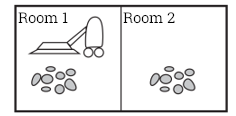
\includegraphics[width=\textwidth]{img/vacum.png}
%     \end{figure}
% \end{minipage}
% \begin{minipage}[t]{0.8\textwidth}
%     An Example for planning $l\;\{h1(:b1); h2(:b2), \ldots\}\;u$

%     \begin{itemize}
%         \item $move(A,B,T)$ :- $at(A,T), room(B)$
%         \item $suck(T)$ :- $at(A,T), dirty(A,T)$
%         \item Init:$at(room1,0), dirty(room1,0), dirty(room2,0)$
%         \item KB=$\{at(room1,0), dirty(room1,0), dirty(room2,0),move(room1,room2,0), suck(0)\}$
%     \end{itemize}
% \end{minipage}

ASP implements a fragment of FOL. We may need some temporal expressiveness in a planning domain.

$X\varphi$ is expressed as $at(B,T+1)$ :- $move(A,B,T)$

The robot's location does not change \textbf{until} it moves, $at(A)\; U\;move(A,B), A!=B$



\tikzset{every picture/.style={line width=0.75pt}} %set default line width to 0.75pt        

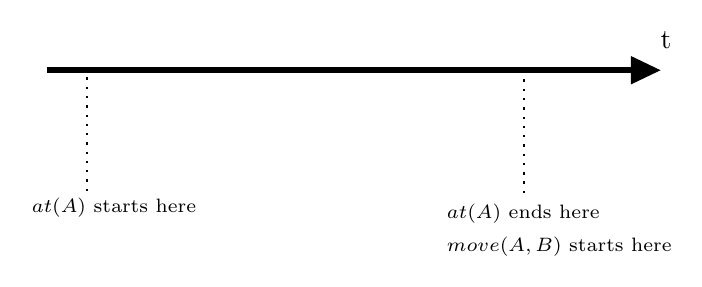
\begin{tikzpicture}[x=0.75pt,y=0.75pt,yscale=-1,xscale=1]
%uncomment if require: \path (0,469); %set diagram left start at 0, and has height of 469

%Straight Lines [id:da6944126603890698] 
\draw [line width=2.25]    (131,92) -- (421.42,92) ;
\draw [shift={(426.42,92)}, rotate = 180] [fill={rgb, 255:red, 0; green, 0; blue, 0 }  ][line width=0.08]  [draw opacity=0] (14.29,-6.86) -- (0,0) -- (14.29,6.86) -- cycle    ;
%Straight Lines [id:da04455549601993869] 
\draw  [dash pattern={on 0.84pt off 2.51pt}]  (150,91) -- (150,153.08) ;
%Straight Lines [id:da3086215716473073] 
\draw  [dash pattern={on 0.84pt off 2.51pt}]  (360.71,92) -- (360.71,154.08) ;

% Text Node
\draw (122,152) node [anchor=north west][inner sep=0.75pt]   [align=left] {{\scriptsize $\displaystyle at( A)$ starts here}};
% Text Node
\draw (322,155) node [anchor=north west][inner sep=0.75pt]   [align=left] {{\scriptsize $\displaystyle at( A)$ ends here}\\{\scriptsize $\displaystyle move( A,B)$ starts here}};
% Text Node
\draw (425,72) node [anchor=north west][inner sep=0.75pt]   [align=left] {t};

\end{tikzpicture}

\begin{itemize}
    \item $at(A,T)$ :- $init(at(A),T)$
    \item $at(A,T)$ :- $at(A,T-1), not\; term(at(A),T)$
    \item $move(A,B,T)$ :- $init(move(A,B),T)$
\end{itemize}

Instead of saying until we say at time $t$ something starts holding, until something else occurs it holds.
In between it continues holding.

This assumption is called $INERTIA$

\subsubsection{ASP reasoning}
So far, we have seen main syntax and semantics of ASP.

How do we perform reasoning in ASP? Hence, how can an ASP program actually produce a plan?

To this there exist two main phases:
\begin{itemize}
    \item Grounding
    \item Solving (reasoning in propositional logic)
\end{itemize}

\textbf{Grounding}

Apply a substitution to variables, depending on initial conditions and propagating through axioms (let's do it for $T<2$ for simplicity).\\

$room(room1;room2)$\\
$at(room1,0)$\\
$closed\_door(0)$\\
$move(A,B,T)$ :- $at(A,T), room(B)$\\
$init(at(A),T)$ :- $move(B,A,T-1)$\\
$term(at(A),T)$ :- $move(A,B,T-1), A\ne B$\\
$at(A,T)$ :- $init(at(A),T)$\\
$at(A,T)$ :- $at(A,T-1), not term(at(A),T)$\\
:- $move(A,B,T), closed\_door(T)$\\
:- $not\;at(room2,1)$ (GOAL AS CONSTRAINT)\\

Substitute
$A=room1,\;B=room2,\;T=0,1$\\

$room(room1)\;room(room2)$\\
$at(room1,0)$\\
$closed\_door(0)$\\
$move(room1,room2,0) \leftarrow at(room1,0), room(room2)$\\
$init(at(room2),1) \leftarrow move(room2,room1,0)$\\
$term(at(room1),1)  \leftarrow move(room1,room2,0), room1\ne room2$\\
$at(room2,0)$ :- $init(at(room2),1)$\\
$Falsum \leftarrow move(room1, room2,0), closed\_door(0)$\\
$Falsum \leftarrow not\;at(room2, 1)$\\

Ground atoms become True Booleans (facts)! The set of all possible groundings is also known as Herbrand universe of program.

\newpage
The goal of an answer set solver, given a ground program, is to compute the answer sets (or stable models) of it.

Given a ground knowledge base KB, a \textbf{stable model} of KB is a \textbf{minimal set} of True Booleans (facts) \textbf{satisfying} KB.

\subsubsection{ASP reasoning in practice}
In practice Solving is an instance of Conflict-Driven Constraint Learning for SAT checkin.

Grounding is Exp Time Hard and its one of the main bottleneks, there are some assumptions that help
mitigating the complexity like Safe Axioms which helps reducing the number of possible groundings.